\section*{Результаты измерений}

\subsection*{Определение цены деления предметной шкалы}

Определим цену деления предметной шкалы транспаранта.

Установив транспарант вблизи зелёного лазера с длиной волны $\lambda = 523 \nm$, наблюдаем дифракционную картину на экране, расположенном на расстоянии $L = 1062 \pm 5 \mm$ от транспаранта. Расстояние измерялось стальной линейкой, но так как рейтеры не были расположены на оптическом рельсе, и линейка была короче измеряемого расстояния (было проведено два измерения) то погрешность оценим как $\sigma_L=5 \mm$.

Было измерено расстояние между дифракционными максимумами на экране $\Delta x = 5 \pm 0.5 \mm$. Измерения проводились стальной линейкой. Погрешность измерения определяется погрешностью отсчёта $\sigma_{дел} = 0.5 \mm$ и инструментальной погрешностью линейки $\sigma_{инстр} = 0.1 \mm$. Итоговая погрешность $\sigma_{\Delta x} = \sqrt{\sigma_{дел}^2 + \sigma_{инстр}^2} = 0.5 \mm$.

Цену деления определим по формуле дифракции Фраунгофера на препятствии:
$$D = \frac{L}{\Delta x} \lambda = 111 \pm 11 \um$$

Определим цену деления шкалы вторым способом.

Поместим после транспаранта положительную линзу с фокусным расстоянием $f = 43 \mm$ и получим на экране сфокусированное увеличенное изображение предметной шкалы. \\
Расстояние от транспаранта до линзы $a = 51 \pm 0.5 \mm$. \\
Расстояние от линзы до экрана $b = 1011 \pm 5 \mm$. \\
На экране наблюдалось 8 делений шкалы. Размер $N = 8$ делений $d = 19 \pm 0.5 \mm$.
По формуле увеличения тонкой линзы определим цену деления шкалы предмета: $$D = \frac{d}{N} \cdot \frac{b}{a} = 119 \pm 3 \um$$

Второй способ точнее, так как на экране наблюдается изображение, геометрические размеры которого измеряются точнее, чем в первом способе.

\subsection*{Определение расстояния от точечного источника до голограммы методом наблюдения интерференционной картины на экране}

Определим расстояние от голограммы до точечного источника, использованного при её создании.

Осветим голограмму лазером, после голограммы с помощью линзы с фокусным расстоянием $f = 43 \mm$ получим увеличенное изображение интерференционной картины. Измерим радиусы тёмных колец. \\
\begin{tabular}{|c|c|c|c|c|c|c|c|c|}
	\hline
	№ & 1 & 2 & 3 & 4 & 5 & 6 & 7 & 8 \\
	\hline
	$r_n, \mm$ & 2 & 3.5 & 4.5 & 5.5 & 6 & 7 & 7.5 & 8 \\
	\hline
\end{tabular}

Построим график зависимости квадрата радиуса тёмного кольца от его номера $r^2(n)$.

\begin{figure}[H]
	\centering
	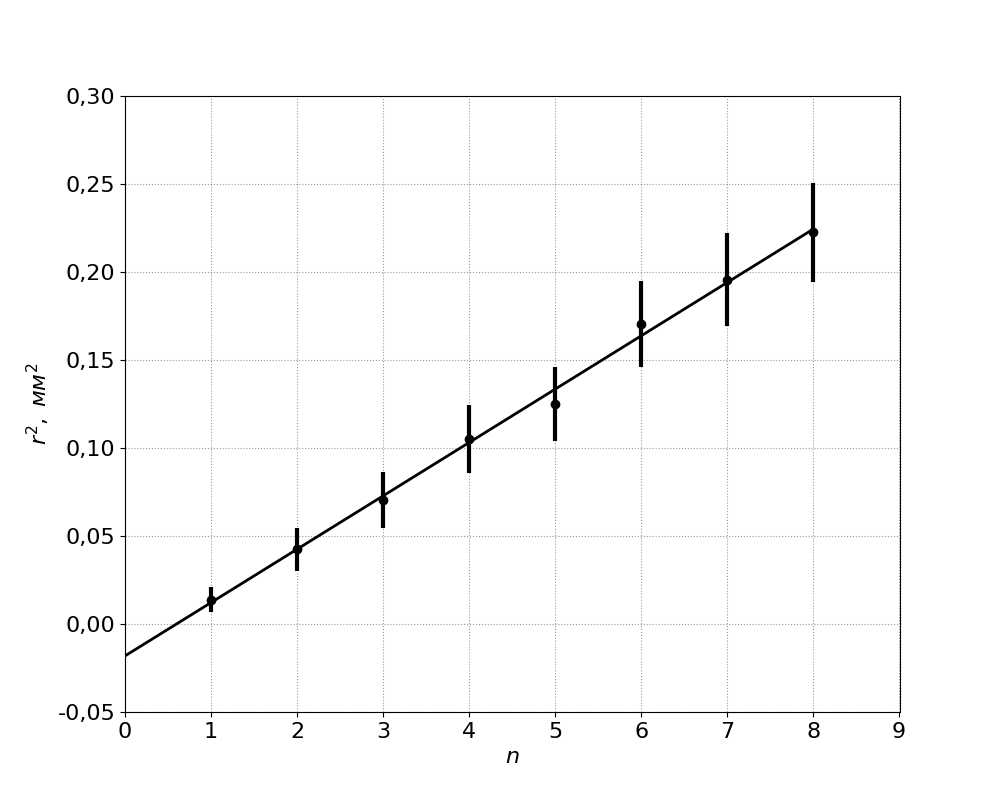
\includegraphics[width=0.6\textwidth]{../Графики/rho_n.png}
	\caption{График зависимости $r^2(n)$}
\end{figure}

Теоретический радиус тёмных колец определяется по формуле:
$$
r_n^2 = n \lambda z_0
$$
Аппроксимируем полученную зависимость прямой $y = ax + b$ и определим расстояние от голограммы до источника $z_0$.

Коэффициенты аппроксимирующей прямой:\\
$a = (30,3 \pm 0,7) \cdot 10^{-3} \; мм^2$ \\
$b = (-18 \pm 4) \cdot 10^{-3} \; мм^2$ \\

Определим расстояние от голограммы до точечного источника: \\
$z_0 = 5,8 \pm 0,1 \cm$.

\subsection*{Определение расстояния до мнимого и действительного изображений}

Определим расстояние до действительного и мнимого изображений голограммы. \\
$b$ -- расстояние от экрана до линзы. \\
$a$ -- расстояние от линзы до голограммы. \\
$d$ -- модуль расстояния от голограммы до изображения точеного источника.

\begin{tabular}{|c|c|c|c|}
	\hline
	Изображение & $a, \mm$ & $b, \mm$ & $d, \mm$ \\
	\hline
	\multicolumn{4}{|c|}{Падение лучей под углом} \\
	\hline
	Действительное & 133 & 692 & $45,1 \pm 0,7$ \\
	Мнимое & 65 & 760 & $21,9 \pm 0,7$\\
	\hline
	\multicolumn{4}{|c|}{Падение лучей под углом} \\
	\hline
	Действительное & 136 & 643 & $47,2 \pm 0,7$ \\
	Мнимое & 69 & 710 & $18,6 \pm 0,7$ \\
	\hline
\end{tabular}

Погрешность измерения расстояний $a$, $b$ равна $0,5$.
Значения расстояния от мнимого и действительно изображений до голограммы, и расстояние от точечного источника до голограммы не совпадают из-за допущенной в ходе эксперимента ошибки: на экране была получена интерференционная картина не голограммы. Предметная шкала давала чёткое изображение на экране на расстоянии $L = 1062 \mm$, расстояние от транспаранта до линзы $a = 51$, расстояние от линзы до экрана $b = 1011$. Транспарант с голограммой был расположен на расстоянии $L' = 826 \mm$, $a = 46 \mm$, $b = 780 \mm$.

\subsection*{Определение фокусирующих свойств голограммы}

С помощью фокусирующих свойств голограммы определим расстояние от голограммы до предметной шкалы $a$. Расстояние от голограммы до экрана $b = 800 \pm 5 \mm$. Размер деления на экране $D' = 2,3 \pm 0,2 \mm$. Расстояние до предмета:
$$
a = b \frac{D}{D'} = 3,8 \pm 0,5 \cm
$$
По формуле тонкой линзы определим фокусное расстояние и оптическую силу голограммы: \\
$$f^{-1} = \frac{1}{a} + \frac{1}{b} = 3,88 \pm 0,03 \; дптр$$
$$f = \frac{1}{f^{-1}} = 25,8 \pm 0,2 \cm$$

Итого расстояние от точечного источника до голограммы $z_0 = 38 \pm 5 \mm$.

\subsection*{Исследование свойств голограммы объёмного предмета}

В работе был измерен угол падения опорной волны, использованной при создании голограммы $\varphi = 47^\circ$.

Было проверено свойство голограммы: при закрытии её части непрозрачным листом бумаги, изображение полностью восстанавливалось по оставшейся открытой части.

Было измерено расстояние от голограммы до предметов, использованных при её создании:
Расстояние до линейки $l_1 = 101 \mm$. \\
Расстояние до гвоздя $l_2 = 151 \mm$.